\documentclass[11pt,aspectratio=169,notheorems]{beamer}

%%%%%%%%%%%%%%%%%%%%%%%%%%%%%%%%%%%%%%%%%%%%%%%%%%%%%%%
% Grundlagen
%%%%%%%%%%%%%%%%%%%%%%%%%%%%%%%%%%%%%%%%%%%%%%%%%%%%%%%
\usepackage{savesym}
\usepackage[ngerman]{babel}
\usepackage{hyperref}

\usepackage{etoolbox}

% Icons
\usepackage[scale=2]{ccicons}
% Glyphen
\usepackage{wasysym}

\usepackage{bookmark}
\usepackage{booktabs}

% Mathe Symbole
\usepackage{stmaryrd}
\usepackage{amssymb}
\usepackage{amsmath}
\savesymbol{iint}
\usepackage[style=english]{csquotes}
\usepackage[style=alphabetic]{biblatex}
%%%%%%%%%%%%%%%%%%%%%%%%%%%%%%%%%%%%%%%%%%%%%%%%%%%%%%%



%%%%%%%%%%%%%%%%%%%%%%%%%%%%%%%%%%%%%%%%%%%%%%%%%%%%%%%
% Logik
%%%%%%%%%%%%%%%%%%%%%%%%%%%%%%%%%%%%%%%%%%%%%%%%%%%%%%%
\usepackage{prftree}
%%%%%%%%%%%%%%%%%%%%%%%%%%%%%%%%%%%%%%%%%%%%%%%%%%%%%%%



%%%%%%%%%%%%%%%%%%%%%%%%%%%%%%%%%%%%%%%%%%%%%%%%%%%%%%%
% Grafik
%%%%%%%%%%%%%%%%%%%%%%%%%%%%%%%%%%%%%%%%%%%%%%%%%%%%%%%
\usepackage{pgfplots}
\usepackage{tikz}
\usetikzlibrary{shapes.symbols}
\usepackage{transparent}
\usepackage{caption}
\usepackage{graphicx}
%%%%%%%%%%%%%%%%%%%%%%%%%%%%%%%%%%%%%%%%%%%%%%%%%%%%%%%



%%%%%%%%%%%%%%%%%%%%%%%%%%%%%%%%%%%%%%%%%%%%%%%%%%%%%%%
% Typografie
%%%%%%%%%%%%%%%%%%%%%%%%%%%%%%%%%%%%%%%%%%%%%%%%%%%%%%%
\usepackage{siunitx}
\usepackage{xspace}
\usepackage{pxfonts}
\restoresymbol{PXF}{iint}
\usepackage{eulervm}
\usepackage{fontawesome}
\usepackage{tcolorbox}
%%%%%%%%%%%%%%%%%%%%%%%%%%%%%%%%%%%%%%%%%%%%%%%%%%%%%%%



%%%%%%%%%%%%%%%%%%%%%%%%%%%%%%%%%%%%%%%%%%%%%%%%%%%%%%%
% Algorithmen und Code
%%%%%%%%%%%%%%%%%%%%%%%%%%%%%%%%%%%%%%%%%%%%%%%%%%%%%%%
\usepackage{algorithm}
\usepackage[noend]{algpseudocode}
%%%%%%%%%%%%%%%%%%%%%%%%%%%%%%%%%%%%%%%%%%%%%%%%%%%%%%%



%%%%%%%%%%%%%%%%%%%%%%%%%%%%%%%%%%%%%%%%%%%%%%%%%%%%%%%
% Beamer
%%%%%%%%%%%%%%%%%%%%%%%%%%%%%%%%%%%%%%%%%%%%%%%%%%%%%%%
\usepackage{appendixnumberbeamer}
%%%%%%%%%%%%%%%%%%%%%%%%%%%%%%%%%%%%%%%%%%%%%%%%%%%%%%%
%%%%%%%%%%%%%%%%%%%%%%%%%%%%%%%%%%%%%%%%%%%%%%%%%%%%%%%
% Grundlagen Farben
%%%%%%%%%%%%%%%%%%%%%%%%%%%%%%%%%%%%%%%%%%%%%%%%%%%%%%%
\definecolor{maincolor}{rgb}{0,0.31,0.62}
\colorlet{maincolorDark}{maincolor!80!black}
\colorlet{maincolorMedium}{maincolor!50!white}
\colorlet{maincolorLight}{maincolor!20!white}
\colorlet{maincolorExtraLight}{maincolor!10!white}
\colorlet{maincolorExtraExtraLight}{maincolor!5!white}
\definecolor{cec1d24}{RGB}{236,29,36}
\definecolor{cffffff}{RGB}{255,255,255}

\hypersetup{
    colorlinks,
    citecolor=maincolor,
    filecolor=black,
    linkcolor=maincolorDark,
    urlcolor=maincolorDark
}

%% Typentheorie Farben
\definecolor{typecolor}{HTML}{0101FD}
\definecolor{termcolor}{HTML}{007D9A}
\definecolor{contextcolor}{HTML}{888888}
\definecolor{universecolor}{HTML}{A139B7}

%%%%%%%%%%%%%%%%%%%%%%%%%%%%%%%%%%%%%%%%%%%%%%%%%%%%%%%



%%%%%%%%%%%%%%%%%%%%%%%%%%%%%%%%%%%%%%%%%%%%%%%%%%%%%%%
% Komplexitätsklassen
%%%%%%%%%%%%%%%%%%%%%%%%%%%%%%%%%%%%%%%%%%%%%%%%%%%%%%%
\newcommand{\class}[1]{\ensuremath{\mathsf{#1}}\xspace}

%% Maße
\newcommand{\TIME}{\class{TIME}}
\newcommand{\SPACE}{\class{SPACE}}
\newcommand{\NTIME}{\class{NTIME}}
\newcommand{\NSPACE}{\class{NSPACE}}

%% Polynomial
\newcommand{\DP}{\class{P}}
\newcommand{\NP}{\class{NP}}

%% PH
\newcommand{\PH}{\class{PH}}

%% Probabilistic
\newcommand{\PP}{\class{PP}}
\newcommand{\ZPP}{\class{ZPP}}
\newcommand{\BPP}{\class{BPP}}
\newcommand{\RP}{\class{RP}}
%%%%%%%%%%%%%%%%%%%%%%%%%%%%%%%%%%%%%%%%%%%%%%%%%%%%%%%



%%%%%%%%%%%%%%%%%%%%%%%%%%%%%%%%%%%%%%%%%%%%%%%%%%%%%%%
% Typentheorie
%%%%%%%%%%%%%%%%%%%%%%%%%%%%%%%%%%%%%%%%%%%%%%%%%%%%%%%
\newcommand{\Type}[1]{{\color{typecolor}\ensuremath{#1}}\xspace}
\newcommand{\Term}[1]{{\color{termcolor}\ensuremath{#1}}\xspace}
\newcommand{\Context}[1]{{\color{contextcolor}\ensuremath{#1}}\xspace}
\newcommand{\Universe}[1]{{\color{universecolor}\ensuremath{\mathcal{U}_{#1}}}\xspace}
%%%%%%%%%%%%%%%%%%%%%%%%%%%%%%%%%%%%%%%%%%%%%%%%%%%%%%%


%%%%%%%%%%%%%%%%%%%%%%%%%%%%%%%%%%%%%%%%%%%%%%%%%%%%%%%
% Typografie
%%%%%%%%%%%%%%%%%%%%%%%%%%%%%%%%%%%%%%%%%%%%%%%%%%%%%%%

% Math und Text bold
\newcommand\allbold[1]{{\boldmath\textbf{#1}}}

% Box
\newtcolorbox{simplebox}{
    colback=maincolorExtraExtraLight,
    colframe=maincolorExtraLight,
    sharpish corners
    }

% Theorem Environments
\tcbuselibrary{theorems, skins}

\makeatletter
\newtcbtheorem[]{definition}{Definition}{
  enhanced,
  colback=maincolorExtraExtraLight,
  coltitle=black,
  colframe=maincolorMedium,
  fonttitle=\large\bfseries,
  description delimiters parenthesis,
  sharpish corners,
  attach boxed title to top,
  boxed title style={colframe=maincolorMedium, colback=maincolorLight, sharpish corners, boxrule=0.5mm},
  toptitle=0.7mm,
  enlarge top by=0.4cm,
  bottomtitle=0.5mm}{def}

\newtcbtheorem[use counter from=definition]{theorem}{Satz}{
  enhanced,
  colback=maincolorExtraExtraLight,
  coltitle=black,
  colframe=maincolorMedium,
  fonttitle=\large\bfseries,
  description delimiters parenthesis,
  sharpish corners,
  attach boxed title to top,
  boxed title style={colframe=maincolorMedium, colback=maincolorLight, sharpish corners, boxrule=0.5mm},
  toptitle=0.7mm,
  enlarge top by=0.4cm,
  bottomtitle=0.7mm}{thm}

\newtcbtheorem[use counter from=definition]{example}{Beispiel}{
  enhanced,
  coltitle=maincolor,
  colback=maincolorExtraExtraLight,
  colframe=maincolorExtraLight,
  fonttitle=\large\bfseries,
  description delimiters parenthesis,
  sharpish corners,
  detach title,
  before upper={\tcbtitle\par},
  enlarge top by=0.4cm}{example}

  \newtcbtheorem[number within=chapter, use counter from=definition]{lemma}{Lemma}{
    enhanced,
    coltitle=maincolor,
    colback=maincolorExtraExtraLight,
    fonttitle=\bfseries,
    sharpish corners,
    colframe=maincolorExtraExtraLight,
    detach title,
    before upper={\tcbtitle\quad},
    enlarge top by=0.4cm}{lemma}
\makeatother

\renewcommand\qedsymbol{\color{maincolor}$\blacksquare$}

\newcommand\hmmax{0}
\newcommand\bmmax{0}
%%%%%%%%%%%%%%%%%%%%%%%%%%%%%%%%%%%%%%%%%%%%%%%%%%%%%%%



%%%%%%%%%%%%%%%%%%%%%%%%%%%%%%%%%%%%%%%%%%%%%%%%%%%%%%%
% Algorithmen und Code
%%%%%%%%%%%%%%%%%%%%%%%%%%%%%%%%%%%%%%%%%%%%%%%%%%%%%%%

% Kommentare
\renewcommand\algorithmiccomment[1]{%
  \allbold{\color{maincolorDark}\hfill$\triangleright$\ #1}
}

% Keywords
\newcommand\Accept{\textbf{accept}}
\newcommand\Reject{\textbf{reject}}

\algnewcommand\algorithmicOutput{\textbf{Output:}}
\algnewcommand\Output{\item[\algorithmicOutput]}
\algnewcommand\algorithmicInput{\textbf{Input:}}
\algnewcommand\Input{\item[\algorithmicInput]}

%%%%%%%%%%%%%%%%%%%%%%%%%%%%%%%%%%%%%%%%%%%%%%%%%%%%%%%



%%%%%%%%%%%%%%%%%%%%%%%%%%%%%%%%%%%%%%%%%%%%%%%%%%%%%%%
% Beamer Style
%%%%%%%%%%%%%%%%%%%%%%%%%%%%%%%%%%%%%%%%%%%%%%%%%%%%%%%
\usetheme[progressbar=head]{metropolis}
\setbeamercolor{frametitle}{bg=black!2, fg=maincolor}
\setbeamerfont{frametitle}{size=\Large}
\setbeamerfont{page number in head/foot}{size=\large}
%\usefonttheme{serif}
%%%%%%%%%%%%%%%%%%%%%%%%%%%%%%%%%%%%%%%%%%%%%%%%%%%%%%%



%%%%%%%%%%%%%%%%%%%%%%%%%%%%%%%%%%%%%%%%%%%%%%%%%%%%%%%
% Special Slides
%%%%%%%%%%%%%%%%%%%%%%%%%%%%%%%%%%%%%%%%%%%%%%%%%%%%%%%
% Section Slide
\newcommand{\sectionslide}[1]{\begin{frame}[noframenumbering]
    \thispagestyle{empty}
    \begin{center}
    \Huge #1
    \end{center}
    \begin{tikzpicture}[overlay, remember picture]
        \node[below right=0cm and 0cm of current page.north west] (tr1_1) {};
        \node[below right=3cm and 0cm of current page.north west] (tr1_2) {};
        \node[below right=0cm and 3cm of current page.north west] (tr1_3) {};

        \fill[fill=maincolorMedium] (tr1_1.center)--(tr1_2.center)--(tr1_3.center);

        \node[above right=0cm and 0cm of current page.south west] (tr2_1) {};
        \node[above right=0cm and 3cm of current page.south west] (tr2_2) {};
        \node[above right=3cm and 0cm of current page.south west] (tr2_3) {};

        \fill[fill=maincolorMedium] (tr2_1.center)--(tr2_2.center)--(tr2_3.center);

        \node[above left=0cm and 0cm of current page.south east] (tr3_1) {};
        \node[above left=0cm and 3cm of current page.south east] (tr3_2) {};
        \node[above left=3cm and 0cm of current page.south east] (tr3_3) {};

        \fill[fill=maincolor] (tr3_1.center)--(tr3_2.center)--(tr3_3.center);

        \node[below left=0cm and 0cm of current page.north east] (tr4_1) {};
        \node[below left=3cm and 0cm of current page.north east] (tr4_2) {};
        \node[below left=0cm and 3cm of current page.north east] (tr4_3) {};

        \fill[fill=maincolorMedium] (tr4_1.center)--(tr4_2.center)--(tr4_3.center);
    \end{tikzpicture}
\end{frame}}
%%%%%%%%%%%%%%%%%%%%%%%%%%%%%%%%%%%%%%%%%%%%%%%%%%%%%%%



%%%%%%%%%%%%%%%%%%%%%%%%%%%%%%%%%%%%%%%%%%%%%%%%%%%%%%%
% Grafik
%%%%%%%%%%%%%%%%%%%%%%%%%%%%%%%%%%%%%%%%%%%%%%%%%%%%%%%
\usepgfplotslibrary{dateplot}

\usetikzlibrary{mindmap,trees,positioning}
%%%%%%%%%%%%%%%%%%%%%%%%%%%%%%%%%%%%%%%%%%%%%%%%%%%%%%%



%%%%%%%%%%%%%%%%%%%%%%%%%%%%%%%%%%%%%%%%%%%%%%%%%%%%%%%
% Custom Symbols
%%%%%%%%%%%%%%%%%%%%%%%%%%%%%%%%%%%%%%%%%%%%%%%%%%%%%%%
% Mengen
\newcommand{\R}{\ensuremath{\mathbb{R}}}
\newcommand{\Z}{\ensuremath{\mathbb{Z}}}
\newcommand{\N}{\ensuremath{\mathbb{N}}}
\newcommand{\Complex}{\ensuremath{\mathbb{C}}}
\newcommand{\Q}{\ensuremath{\mathbb{Q}}}

% Danger Symbol
\newcommand*{\TakeFourierOrnament}[1]{{%
\fontencoding{U}\fontfamily{futs}\selectfont\char#1}}
\newcommand*{\danger}{\TakeFourierOrnament{66}}

% under construction
\newcommand{\ucmark}{\tikz[y=0.80pt,x=0.80pt,yscale=-0.02,xscale=0.02, inner sep=0pt, outer sep=0pt]%
  {\path[fill=cec1d24,nonzero rule] (635.8833,600.0000) .. controls
    (651.0771,599.6647) and (665.7558,591.6224) .. (673.9783,577.5525) .. controls
    (682.1001,563.3625) and (681.7384,546.6500) .. (674.5074,533.1862) --
    (378.4699,21.6487) .. controls (370.6590,8.7662) and (356.3424,0.0975) ..
    (340.1099,-0.0063) .. controls (323.6499,0.0972) and (309.3362,8.7657) ..
    (301.4862,21.6487) -- (5.4612,533.1862) .. controls (-1.7257,546.6500) and
    (-2.0877,563.3625) .. (5.9903,577.5525) .. controls (14.2570,591.6225) and
    (28.9353,599.6650) .. (44.0853,600.0000) -- (635.8853,600.0000);
    \path[fill=cffffff,nonzero rule] (340.1208,75.7875) -- (71.0683,540.8450) --
    (608.8933,540.8450) -- (340.1058,75.7950);
    \path[fill=black,nonzero rule] (303.5900,225.7800) .. controls
    (280.4500,225.7300) and (276.9200,248.1400) .. (276.8800,250.6200) .. controls
    (276.9200,262.4400) and (285.4000,277.1700) .. (309.1600,279.4100) .. controls
    (309.1600,279.4100) and (313.7700,280.0900) .. (313.6600,283.0900) .. controls
    (313.7700,285.9400) and (313.7800,284.9700) .. (312.3400,286.5300) .. controls
    (310.8500,288.2300) and (298.5500,299.6400) .. (298.3100,302.6600) .. controls
    (296.9800,316.8800) and (300.1800,335.2800) .. (303.0900,345.9400) .. controls
    (303.0900,345.9400) and (306.6000,354.7800) .. (303.8800,361.0000) .. controls
    (301.0600,367.4700) and (289.0000,397.7400) .. (288.0000,399.5600) .. controls
    (285.1300,404.8200) and (284.0000,409.1400) .. (285.8800,415.4100) .. controls
    (284.6600,416.1100) and (264.4700,428.8800) .. (264.4700,428.8800) .. controls
    (264.4700,428.8800) and (261.3500,421.5100) .. (253.5900,419.3800) .. controls
    (245.7000,417.1100) and (239.1800,418.1800) .. (232.7200,405.9100) --
    (226.8800,396.4100) .. controls (226.8800,396.4100) and (225.6700,392.9300) ..
    (219.7500,391.6200) .. controls (213.9300,390.4900) and (206.1000,388.3000) ..
    (202.8100,388.4700) .. controls (198.6100,388.8800) and (195.2200,387.7300) ..
    (189.5900,394.2800) .. controls (185.0800,399.5300) and (112.8800,524.4700) ..
    (112.8800,524.4700) -- (286.4100,524.4700) .. controls (286.4100,524.4700) and
    (290.7100,524.0000) .. (289.5900,519.9700) .. controls (288.2700,516.1900) and
    (267.3800,441.8100) .. (267.3800,441.8100) -- (291.4400,426.7500) .. controls
    (291.4400,426.7500) and (293.3600,429.9900) .. (300.4400,426.7500) .. controls
    (307.3800,423.4800) and (309.9700,421.7500) .. (309.9700,421.7500) .. controls
    (309.9700,421.7500) and (313.9200,421.4900) .. (313.4100,413.0300) .. controls
    (316.1700,411.3100) and (341.9700,395.0600) .. (341.9700,395.0600) .. controls
    (341.9700,395.0600) and (332.8400,417.6000) .. (331.9100,427.5600) .. controls
    (331.2100,437.4600) and (327.6900,504.1200) .. (327.6900,504.1200) .. controls
    (327.6900,504.1200) and (328.1300,509.2200) .. (324.7800,510.2200) .. controls
    (321.2800,511.1700) and (305.7200,515.5000) .. (305.7200,515.5000) .. controls
    (305.7200,515.5000) and (301.3900,516.2100) .. (301.5000,519.7200) .. controls
    (301.3900,523.0400) and (303.0200,524.3400) .. (304.9400,524.4700) .. controls
    (306.9300,524.3400) and (355.7200,524.4700) .. (355.7200,524.4700) .. controls
    (355.7200,524.4700) and (360.7100,525.0000) .. (361.5300,518.4100) .. controls
    (362.3400,511.9900) and (371.5900,445.5000) .. (371.5900,445.5000) .. controls
    (371.5900,445.5000) and (367.5700,444.4500) .. (367.6200,440.5000) .. controls
    (367.5700,436.3200) and (367.5600,433.2000) .. (368.9400,431.5000) .. controls
    (370.1600,429.9500) and (384.8300,413.0400) .. (394.8800,389.5300) .. controls
    (396.4200,386.0300) and (397.5600,389.1300) .. (397.7800,390.0600) .. controls
    (398.2100,390.7500) and (417.2800,442.6600) .. (419.4700,444.7200) .. controls
    (421.8400,446.5600) and (473.3600,488.2300) .. (474.5000,489.0900) .. controls
    (475.6400,489.8600) and (478.9100,492.1100) .. (479.0000,499.3800) .. controls
    (478.9100,506.7600) and (475.9700,512.6300) .. (473.9700,514.9700) .. controls
    (472.0500,517.1900) and (468.8000,520.4500) .. (468.6900,521.8400) .. controls
    (468.8000,523.3800) and (470.2800,524.3400) .. (471.3400,524.4700) .. controls
    (472.5600,524.3400) and (479.2500,524.3400) .. (479.8100,524.4700) .. controls
    (480.5500,524.3400) and (489.3400,525.0100) .. (495.4100,514.1900) .. controls
    (501.7300,503.5300) and (513.1200,484.3400) .. (513.1200,484.3400) .. controls
    (513.1200,484.3400) and (515.5800,480.5600) .. (512.0600,478.2500) .. controls
    (508.4000,476.0100) and (502.7100,474.7100) .. (499.3800,471.1200) .. controls
    (495.8600,467.5500) and (462.9400,429.6400) .. (462.3400,428.8800) .. controls
    (461.9600,428.3400) and (457.7100,423.7600) .. (452.2800,426.2200) .. controls
    (450.7000,424.0900) and (448.8400,421.2200) .. (448.8400,421.2200) .. controls
    (448.8400,421.2200) and (439.4600,364.4600) .. (429.5300,340.4100) .. controls
    (431.8000,339.0000) and (434.8100,336.7200) .. (434.8100,336.7200) .. controls
    (434.8100,336.7200) and (442.7200,343.5500) .. (449.3800,336.4400) .. controls
    (456.0900,329.2300) and (455.6000,329.4100) .. (454.4100,326.1600) .. controls
    (453.3200,322.9000) and (452.8300,321.9100) .. (450.4400,320.5900) .. controls
    (448.2700,319.3000) and (444.5200,315.5500) .. (444.6200,308.9700) .. controls
    (444.5200,302.5400) and (441.7400,284.8000) .. (438.5300,277.2800) .. controls
    (435.5500,269.8300) and (434.5600,261.5500) .. (422.9100,256.4400) .. controls
    (404.4800,248.2100) and (379.8000,243.3100) .. (361.8100,247.9700) .. controls
    (356.8300,249.3000) and (340.8200,261.0500) .. (339.3100,261.9700) .. controls
    (337.8900,262.6800) and (331.6400,265.2600) .. (332.1900,259.8400) .. controls
    (333.4500,247.4700) and (322.7500,225.7300) .. (303.5900,225.7800) --
    cycle(394.8800,275.9700) .. controls (394.8800,275.9700) and
    (408.4700,275.8400) .. (411.5300,276.2200) .. controls (414.3400,276.5000) and
    (416.0300,280.1900) .. (416.0300,280.1900) -- (429.0000,325.8800) --
    (424.2500,328.7800) .. controls (421.5800,323.2700) and (397.9000,287.2600) ..
    (393.0300,280.4700) .. controls (389.9100,276.1000) and (394.8800,275.9700) ..
    (394.8800,275.9700) -- cycle(331.0000,332.8100) .. controls
    (331.5700,332.7900) and (332.2200,332.9700) .. (332.7200,333.2800) .. controls
    (337.8300,336.2000) and (347.5100,344.5400) .. (355.7200,356.0000) .. controls
    (356.7000,357.3200) and (355.7200,361.2800) .. (355.7200,361.2800) --
    (348.5900,376.0600) .. controls (348.5900,376.0600) and (317.8500,395.3700) ..
    (315.5000,396.9100) .. controls (312.9600,398.3000) and (311.5500,396.9300) ..
    (313.9400,393.7500) .. controls (327.6400,375.1200) and (332.7200,353.0000) ..
    (329.5300,335.1200) .. controls (329.2600,333.4800) and (330.0500,332.8500) ..
    (331.0000,332.8100) -- cycle;}}
%%%%%%%%%%%%%%%%%%%%%%%%%%%%%%%%%%%%%%%%%%%%%%%%%%%%%%%



%%%%%%%%%%%%%%%%%%%%%%%%%%%%%%%%%%%%%%%%%%%%%%%%%%%%%%%
% Sonstiges
%%%%%%%%%%%%%%%%%%%%%%%%%%%%%%%%%%%%%%%%%%%%%%%%%%%%%%%

% Bibliografie

\addbibresource{bibliography.bib}
%%%%%%%%%%%%%%%%%%%%%%%%%%%%%%%%%%%%%%%%%%%%%%%%%%%%%%%

%%%%%%%%%%%%%%%%%%%%%%%%%%%%%%%%%%%%%%%%%%%%%%%%%%%%%%%
% Title
%%%%%%%%%%%%%%%%%%%%%%%%%%%%%%%%%%%%%%%%%%%%%%%%%%%%%%%
\title{\Huge{Homotopietypentheorie}}
\subtitle{Oberseminar Theoretische Informatik}
\date{}
\author{Florian Chudigiewitsch}
\institute{Institut für Theoretische Informatik}
\titlegraphic{
\includegraphics[height=10mm]{images/thi}\hspace{92mm}
\includegraphics[height=10mm]{images/logo_luh}}
%%%%%%%%%%%%%%%%%%%%%%%%%%%%%%%%%%%%%%%%%%%%%%%%%%%%%%%

\begin{document}


\begin{frame}[noframenumbering]
    \maketitle
    \thispagestyle{empty}
    \begin{tikzpicture}[overlay, remember picture]
        \node[above left=1cm and .8cm of current page.south east] {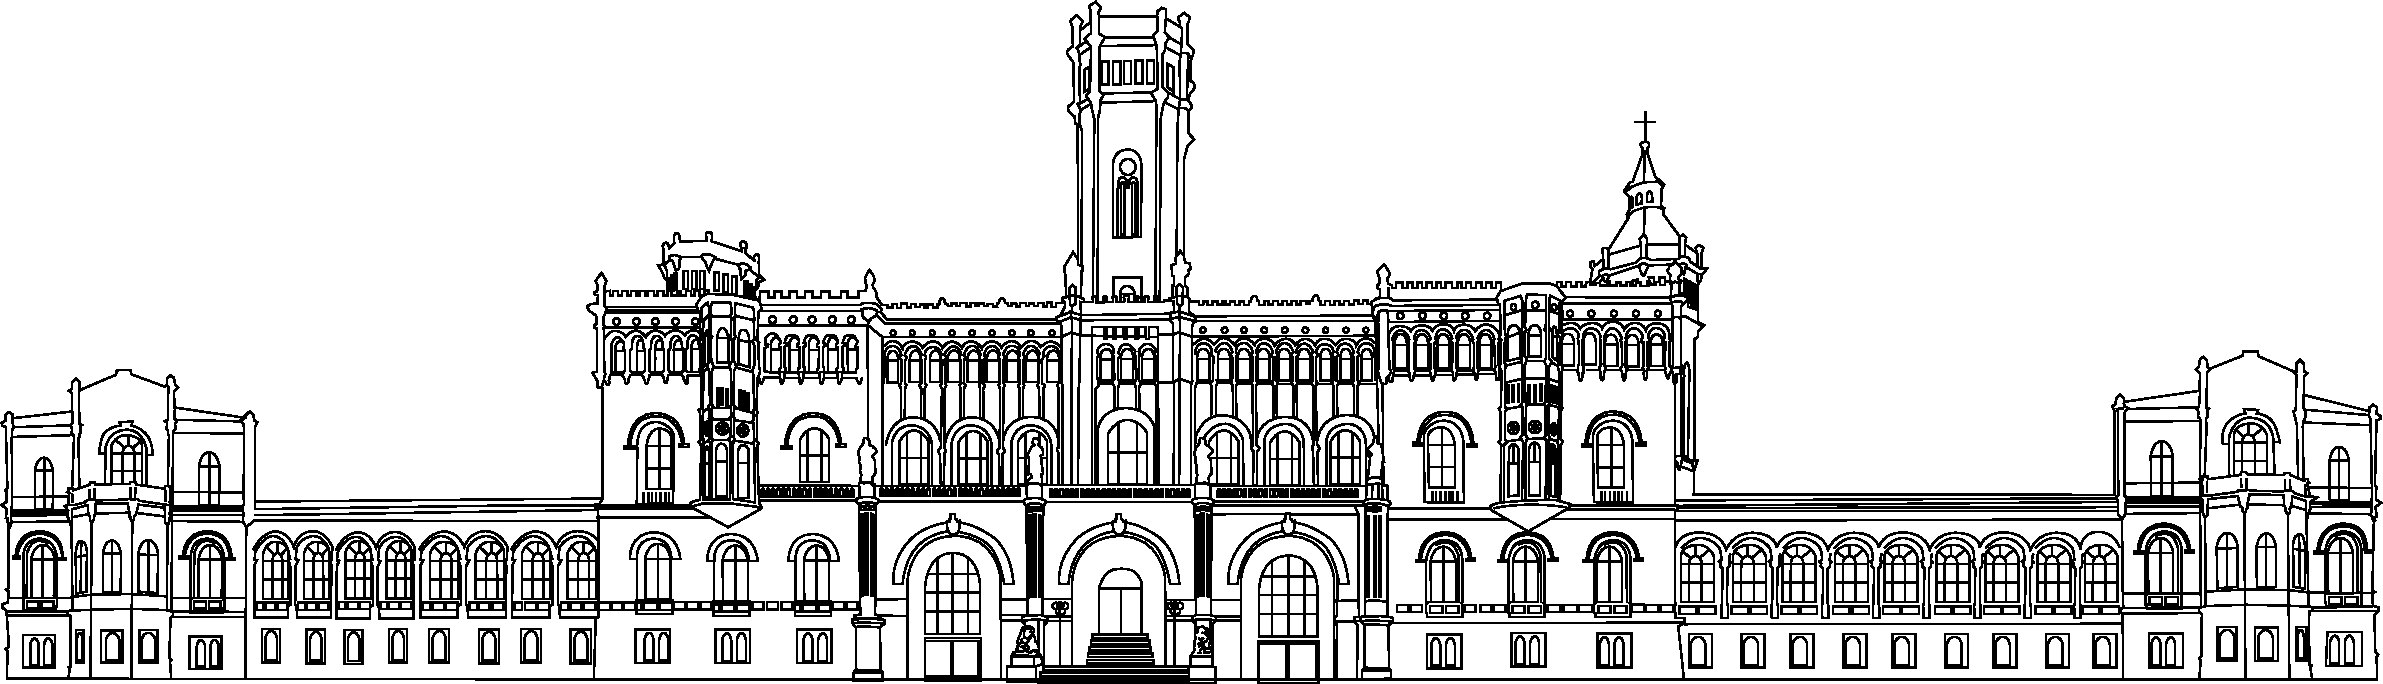
\includegraphics[width=7.5cm]{images/welfenschloss}};
    \end{tikzpicture}
\end{frame}

\begin{frame}[noframenumbering]{Themen}
    \thispagestyle{empty}
    \Large
    \begin{itemize}
        \item Geschichtliches
        \item Grundlagen der Typentheorie
        \item Homotopietypentheorie
        \item Anwendungen \& Aktuelle Forschungsfragen
    \end{itemize}
    
\end{frame}

\sectionslide{Geschichtliches}

\begin{frame}{Geschichtliches}
    \begin{tikzpicture}
        \draw[line width=7pt, maincolorMedium] (0,0) -- (15,0);
        \node[starburst, draw, minimum width=2cm, minimum height=2cm,red,fill=orange,line width=1.5pt]
        {};
        \draw[->, line width=2pt] (0,-2) -- (0,-1);
        \draw (0, -2.5) node {Russellsche Antinomie};
        \draw (0, 1.2) node {1901};


        \uncover<2->{\fill (3.8, -0.2) rectangle (4.2, 0.2);
        \draw[-, line width=2pt] (4,-3) -- (4,0);
        \draw (4, -3.5) node {Dependent Type Theory};
        \draw (4, 1.2) node {1934};}

        
        \uncover<3->{\fill (7.8, -0.2) rectangle (8.2, 0.2);
        \draw[-, line width=2pt] (8,-2) -- (8,0);
        \draw (8, -2.5) node {\href{https://www.math.ias.edu/~vladimir/Site3/Univalent_Foundations_files/Hlambda_short_current.pdf}{Voevodsky Paper}};
        \draw (8, 1.2) node {2006};}

        
        \uncover<4->{\fill (11.8, -0.2) rectangle (12.2, 0.2);
        \draw[-, line width=2pt] (12,-4) -- (12,0);
        \draw (8, -4.5) node {Special Year on Univalent Foundations of Mathematics};
        \draw (12, 1.2) node {2012};}
    \end{tikzpicture}
\end{frame}

\begin{frame}{Quellen und Referenzen}
    \begin{columns}[T] % align columns
        \begin{column}{.30\textwidth}
        \begin{center}
            
\includegraphics[width=0.9\textwidth]{images/cover-web}\\
            \tiny{\href{https://homotopytypetheory.org/book/}{https://homotopytypetheory.org/book/}~\cite{hottbook}}
        \end{center}
        \end{column}%
        \hfill%
        \begin{column}{.30\textwidth}
        \begin{center}
            
\includegraphics[width=0.9\textwidth]{images/computerphile}\\[2pt]
            Computerphile (Youtube)
            \tiny{
            \begin{itemize}
                \item \href{https://www.youtube.com/watch?v=qT8NyyRgLDQ}{Type Theory}
                
                \item \href{https://www.youtube.com/watch?v=SknxggwRPzU}{Propositions as Types}
                
                \item \href{https://www.youtube.com/watch?v=v5a5BYZwRx8}{Voevodsky}
                
                \item \href{https://www.youtube.com/watch?v=Ft8R3-kPDdk}{Homotopy Type Theory}
            \end{itemize}}
        \end{center}
        \end{column}%
        \hfill%
        \begin{column}{.30\textwidth}
        \begin{center}
            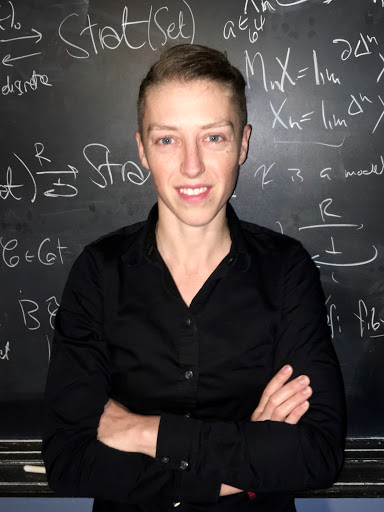
\includegraphics[width=0.9\textwidth]{images/riehl}\\[2pt]
            Emily Riehl
            \tiny{
            \begin{itemize}
                \item \href{http://www.math.jhu.edu/~eriehl/berkeley-logic.mp4}{Video}
                \item \href{http://www.math.jhu.edu/~eriehl/berkeley-logic.pdf}{Slides}
            \end{itemize}}
        \end{center}
        \end{column}%
    \end{columns}
\end{frame}

\sectionslide{Grundlagen der Typentheorie}

\begin{frame}{Konstruktivität}
    \begin{itemize}
        \item Law of excluded middle (LEM) wichtiges Axiom in der klassischen Mathematik
        \item $\vdash \varphi \vee \neg \varphi$
        \item Ermöglicht Widerspruchsbeweise
        \item Konstruktive Logik verzichtet auf LEM
        \item Dadurch wird durch einen Beweis immer ein \glqq{}Witness\grqq{} erzeugt
        \item Keine wirkliche Einschränkung, da man LEM jederzeit als Annahme hinzunehmen kann
    \end{itemize}
\end{frame}

\begin{frame}{Dependent Type Theory: Die vier \glqq{}Grundaussagen\grqq{}}
    Die vier Grundformen (\glqq{}judgements\grqq{}) der \glqq{}wohlgeformten Formeln\grqq{} der Dependent Type Theory sind:
    \begin{center}
        \begin{tabular}{l l l}
            Formel & Interpretation & Beispiel\\ \hline
            $\Context{\Gamma} \vdash \Type{A}$ type & \glqq{}\Type{A} ist ein Typ\grqq{}&\Type{\N} type\\
            $\Context{\Gamma} \vdash \Term{a} : \Type{A}$ & \glqq{}\Term{a} ist ein Term vom Typ \Type{A}\grqq{}&$\Term{1} : \Type{\N}$\\
            $\Context{\Gamma}, \Term{x} : \Type{A} \vdash \Type{B(x)}$ type & \glqq{}\Type{B(x)} ist eine Typfamilie über \Type{A}\grqq{}&$\Term{n} : \Type{\N} \vdash \Type{\R^n}$ type\\
            $\Context{\Gamma}, \Term{x} : \Type{A} \vdash \Term{b(x)} : \Type{B(x)}$ & \glqq{}\Term{b(x)} ist eine Termfamilie\grqq{}&$\Term{n} : \Type{\N} \vdash \Term{\vec{0}} : \Type{\R^n}$\\
        \end{tabular}
    \end{center}
    \Context{\Gamma} ist der \emph{Kontext}, der die Typen aller vorkommenen Variablen deklariert.

    \emph{Universum:} Typ, dessen Elemente Typen sind. Bilden Hierarchie
    \[\Universe{0} : \Universe{1} : \Universe{2} : \cdots\] 
\end{frame}


\begin{frame}{Dependent Type Theory: Die vier \glqq{}Grundregelarten\grqq{} I}
    
    \begin{itemize}
        \item Name: $x$-formation rules

        \item Beschreibung: Haben wir Typen \Type{A} und \Type{B} gegeben, gibt es einen Produkttypen \Type{A\times B}.

        \item Formal:
        \begin{displaymath}
            \prftree[r]{}
                {\Context{\Gamma} \vdash \Type{A} \text{ type}}
                {\Context{\Gamma} \vdash \Type{B} \text{ type}}
                {\Context{\Gamma} \vdash \Type{A\times B} \text{ type}}
        \end{displaymath}
    \end{itemize}
\end{frame}

\begin{frame}{Dependent Type Theory: Die vier \glqq{}Grundregelarten\grqq{} II}
    
    \begin{itemize}
        \item Name: $x$-introduction rules

        \item Beschreibung: Haben wir Terme $\Term{a} : \Type{A}$ und $\Term{b} : \Type{B}$ gegeben, gibt es einen Term $\Term{(a, b)} : \Type{A\times B}$.

        \item Formal: 
        \begin{displaymath}
            \prftree[r]{}
                {\Context{\Gamma} \vdash \Term{a} : \Type{A}}
                {\Context{\Gamma} \vdash \Term{b} : \Type{B}}
                {\Context{\Gamma} \vdash \Term{(a, b)} : \Type{A\times B}}
        \end{displaymath}
    \end{itemize}
\end{frame}

\begin{frame}{Dependent Type Theory: Die vier \glqq{}Grundregelarten\grqq{} III}
    \begin{itemize}
        \item Name: $x$-elimination rules
        \item Beschreibung: Haben wir einen Term $\Term{p} : \Type{A\times B}$ gegeben, gibt es Terme $\Term{\text{pr}_1(p)} : \Type{A}$ und $\Term{\text{pr}_2(p)} : \Type{B}$.
        \item Formal: 

        \begin{columns}[T] % align columns
            \begin{column}{.30\textwidth}
                \begin{displaymath}
                    \prftree[r]{}
                        {\Context{\Gamma} \vdash \Term{p} : \Type{A\times B}}
                        {\Context{\Gamma} \vdash \Term{\text{pr}_1(p)} : \Type{A}}
                \end{displaymath}
            \end{column}%
            \begin{column}{.30\textwidth}
                \begin{displaymath}
                    \prftree[r]{}
                        {\Context{\Gamma} \vdash \Term{p} : \Type{A\times B}}
                        {\Context{\Gamma} \vdash \Term{\text{pr}_2(p)} : \Type{B}}
                \end{displaymath}
            \end{column}%
        \end{columns}
    \end{itemize}
    \vspace{0.5cm}
    \textbf{Weiterhin:} \emph{Judgemental equality ($\alpha$-conversion)}, \emph{computation rules ($\beta$-reduction):} verbinden introduction und elimination rules, optionales \emph{uniqueness principle ($\eta$-expansion)}.
\end{frame}

\begin{frame}{Funktionstypen}
    \begin{itemize}
        \item $\rightarrow$-formation: Haben wir Typen \Type{A} und \Type{B} gegeben, gibt es einen Typen \Type{A\rightarrow B}.
        \item $\rightarrow$-introduction: Haben wir im Kontext eines Terms $\Term{x} : \Type{A}$ einen Term $\Term{b(x)} : \Type{B}$ gegeben, gibt es einen Term $\Term{\lambda x.b(x)} : \Type{A\rightarrow B}$. Formal:
        \begin{displaymath}
            \prftree[r]{}
                {\Context{\Gamma}, \Term{x} : \Type{A} \vdash \Term{b(x)} : \Type{B}}
                {\Context{\Gamma} \vdash \Term{\lambda x.b(x)} : \Type{A\rightarrow B}}
        \end{displaymath}
        \item $\rightarrow$-elimination: Haben wir Terme $\Term{f} : \Type{A\rightarrow B}$ und $\Term{a} : \Type{A}$ gegeben, gibt es einen Term $\Term{f(a)} : \Type{B}$.
        \item Zwei computation rules.
    \end{itemize}
\end{frame}

\begin{frame}{Propositions as Types}
    \begin{itemize}
        \item Aussagen werden durch Typen repräsentiert
        \item Man beweist sie indem man einen Term vom entsprechenden Typ erzeugt
        \item \[\frac{\text{Beweise}}{\text{Aussagen}} = \frac{\text{Programme}}{\text{Typen}}\]
        \item Klassisch: $\text{Prop} \leftrightsquigarrow \text{Bool}$, \glqq{}Wahrheit\grqq{}
        \item Andere Möglichkeit: $\text{Prop} \leftrightsquigarrow \text{Types}$, \glqq{}Zeugnis\grqq{}
    \end{itemize}
\end{frame}

\begin{frame}{Propositions as Types: Beispiel}
    \begin{example}{}{}
        \textbf{Aussage:} Für beliebige Typen \Type{P} und \Type{Q} gibt es den Term \[\Term{\text{modus-ponens}} : \Type{P\times (P\rightarrow Q) \rightarrow Q}.\]

        \textbf{Beweis:} Mit $\rightarrow$-introduction aus Term $\Term{x} : \Type{P\times (P\rightarrow Q)}$ einen Term aus \Type{Q} generieren. $x$-elimination liefert uns $\Term{\text{pr}_1(x)} : \Type{P}$ und $\Term{\text{pr}_2(x)} : \Type{P\rightarrow Q}$.\\$\rightarrow$-elimination liefert $\Term{(\text{pr}_2(x))(\text{pr}_1(x))} : \Type{Q}$.

        Somit: $\Term{\text{modus-ponens}} :\equiv \Term{\lambda x.(\text{pr}_2(x))(\text{pr}_1(x))}$.\hfill{\color{maincolor}$\blacksquare$}
    \end{example}
    \emph{Curry-Howard-Isomorphismus:} Ein Beweis korrespondiert zu einem Computerprogramm, welches einen Term vom Typ der Aussage zurückgibt.
\end{frame}

\begin{frame}{Gleichheit als Identitätstyp}
    Mathematische Gleichheit wird über Identitätstypen ausgedrückt.

    \begin{itemize}
        \item $=$-formation: Haben wir einen Typ \Type{A} und zwei Terme $\Term{x},\Term{y} : \Type{A}$ gegeben, gibt es einen Typ $\Type{x =_{A} y}$.
        \item $=$-introduction: Haben wir einen Term $\Term{x}:\Type{A}$ gegeben, so gibt es einen Term $\Term{\text{refl}_x} : \Type{x =_{A} x}$.
    \end{itemize}
    Elimination rule via path induction:
    
    Haben wir eine Typfamilie $\Context{\Gamma}, \Term{x}, \Term{y} : \Type{A}, \Term{p} : \Type{x =_{A} y} \vdash \Type{B(x, y, p)}$ gegeben und wollen einen Term von \Type{B(x, y, p)} konstruieren, reicht es anzunehmen, dass \Term{y} \Term{x} und \Term{p} \Term{\text{refl}_x} ist.
\end{frame}

\begin{frame}{Gleichheit ist eine Äquivalenzrelation}
    \begin{lemma}{}{}
        Für beliebige $\Term{x}, \Term{y} : \Type{A}$ gilt $\Type{(x =_A y)\rightarrow (y =_A x)}$.
    \end{lemma}
    \begin{proof}
        Hausaufgabe. $\smiley$
    \end{proof}
    \begin{lemma}{}{}
        Für beliebige $\Term{x}, \Term{y}, \Term{z} : \Type{A}$ gilt $\Type{(x =_A y)\rightarrow ((y =_A z)\rightarrow (x =_A z))}$.
    \end{lemma}
    \begin{proof}
        Hausaufgabe. $\smiley$
    \end{proof}
\end{frame}

\sectionslide{Homotopietypentheorie}

\begin{frame}{Path induction \glqq{}homotopisch\grqq{} interpretiert}
    \begin{columns}[T] % align columns
        \begin{column}{.6\textwidth}
            \begin{itemize}
                \item Typ \Type{A} $\leftrightsquigarrow$ Raum \Type{A}
                \item Term $\Term{a} : \Type{A}$ $\leftrightsquigarrow$ Punkt \Term{a} in \Type{A}
                \item Term $\Term{p} : \Type{x =_{A} y}$ $\leftrightsquigarrow$ Pfad \Term{p} von \Term{x} nach \Term{y} in \Type{A}
                \item Term $\Term{p} : \Type{p =_{x =_{A} y} a}$ $\leftrightsquigarrow$ Homotopie \Term{h} von \Term{p} nach \Term{q} in \Type{A}
            \end{itemize}
        \end{column}%
        \begin{column}{.4\textwidth}
            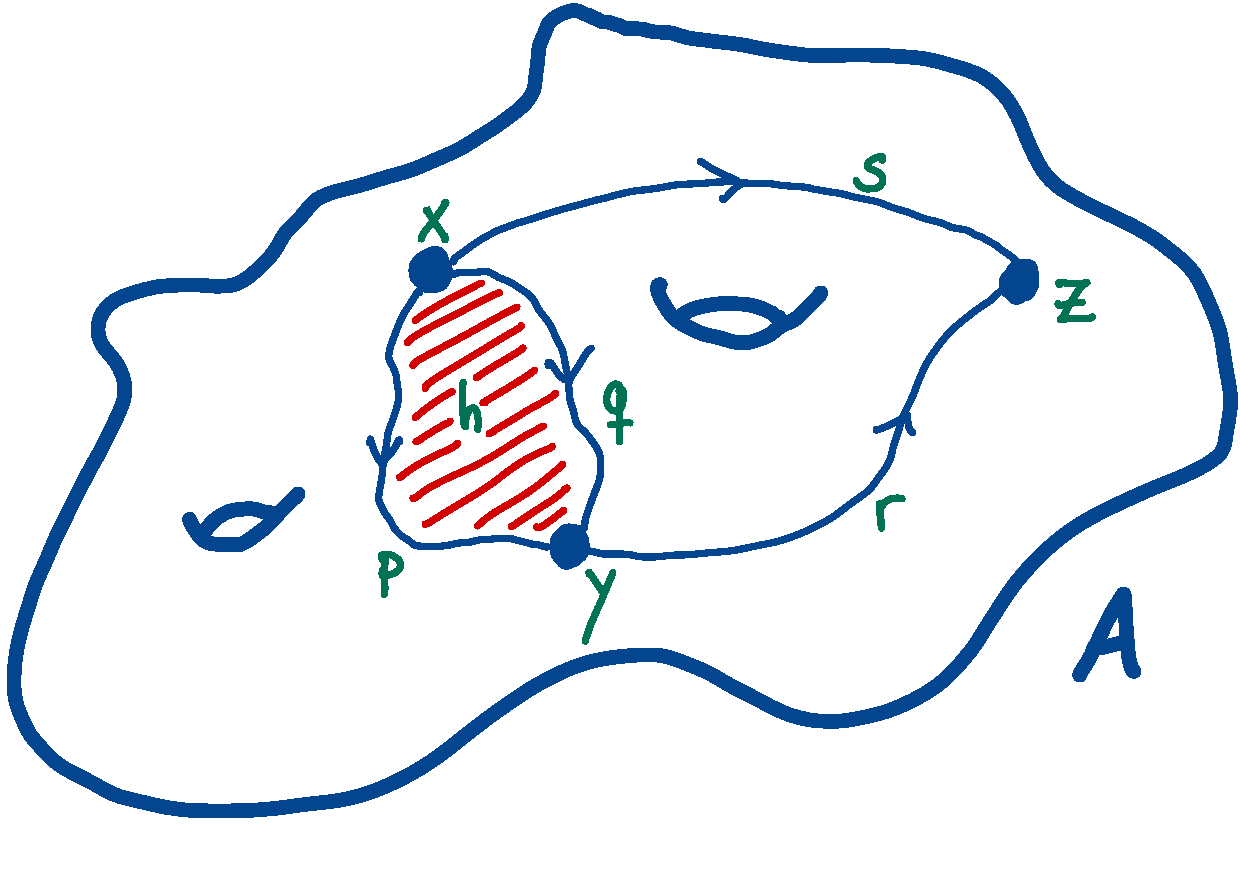
\includegraphics[width=0.95\textwidth]{images/topology1.pdf}
        \end{column}%
    \end{columns}~\\
    \begin{itemize}
        \item Symmetrie und Transitivität wird als Umkehrung und Komposition von Pfaden, Homotopien, höheren Homotopien... interpretiert.
        \item \href{https://arxiv.org/abs/0812.0298}{van den Berg/Garner} und \href{http://peterlefanulumsdaine.com/research/Lumsdaine-2010-Thesis.pdf}{Lumsdaine}: Typen haben die Struktur eines schwachen $\infty$-Gruppoiden
        \item Unterschied: Homotopietheorie analytisch, Homotopietypentheorie synthetisch
    \end{itemize}
\end{frame}

\begin{frame}{\glqq{}Indiscernibility of identicals\grqq{}}
    \textbf{Beantwortete offene Frage der Beweistheorie:}
    \begin{itemize}
        \item \glqq{}Indiscernibility of identicals\grqq{}: Wenn zwei Beweise $p$ und $q$ beide $A$ zeigen, kann man dann immer $p = q$ zeigen?
        \item Nein!
        \item Homotopie-Äquivalenzklassen von Schleifen an einem Punkt $x_0$ bilden die \emph{fundamentale Gruppe}.
    \end{itemize}
    \begin{center}
        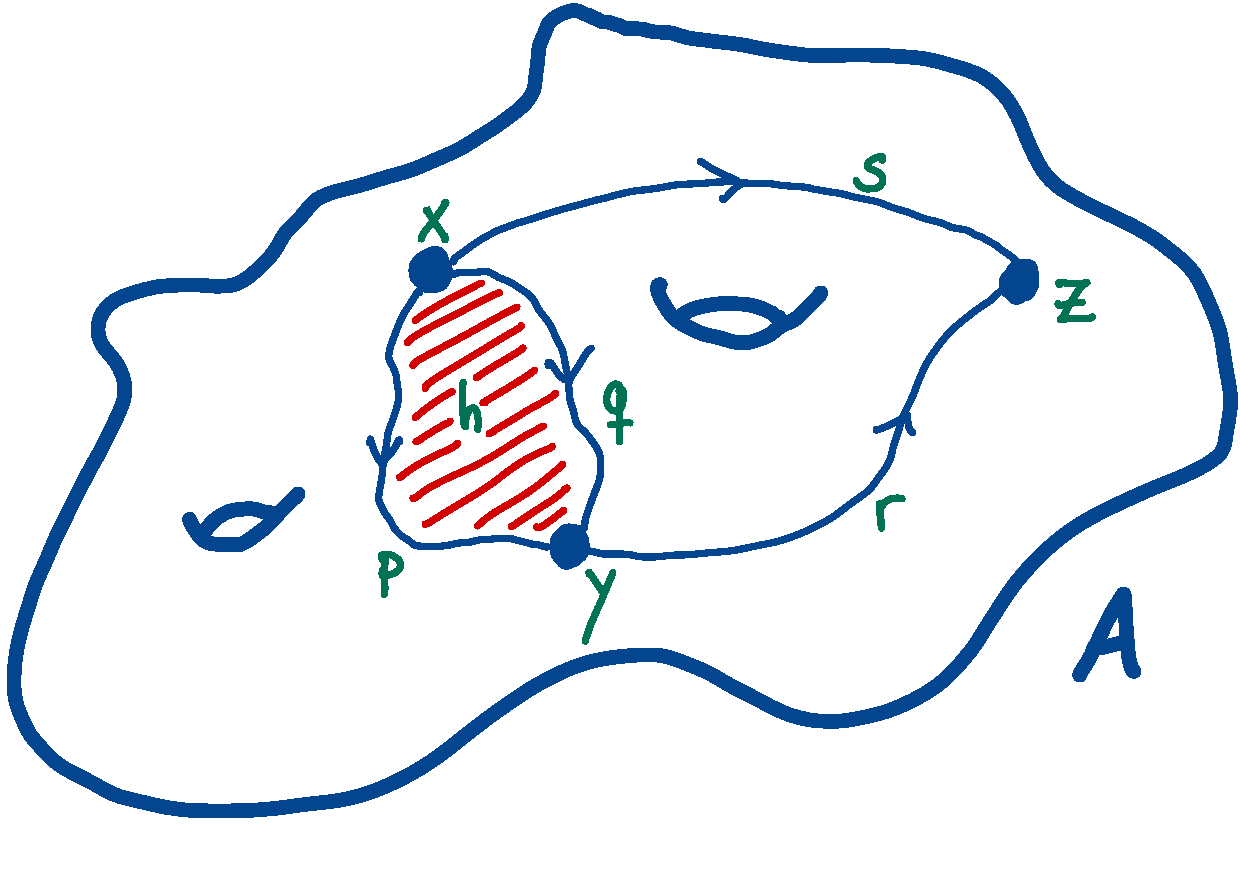
\includegraphics[width=0.35\textwidth]{images/topology1.pdf}
    \end{center}
\end{frame}

\begin{frame}{Weitere Typen -- mit homotopischer Interpretation}
    
    \begin{columns}[T] % align columns
        \begin{column}{.60\textwidth}
            \begin{itemize}
                \item Typfamilie $\Term{x} : \Type{A} \vdash \Type{B(x)}$ type $\leftrightsquigarrow$ Faserung über \Type{A}
                \item Dependent sum Typ \Type{\sum_{x:A} B(x)} $\leftrightsquigarrow$ Totalraum einer Faserung
                
                Beispiel: \[\Type{\text{Gruppoid}} :\equiv \Type{\sum_{A:\Universe{}} (A\rightarrow A \rightarrow A)}\]
            \end{itemize}
        \end{column}%
        \begin{column}{.30\textwidth}
            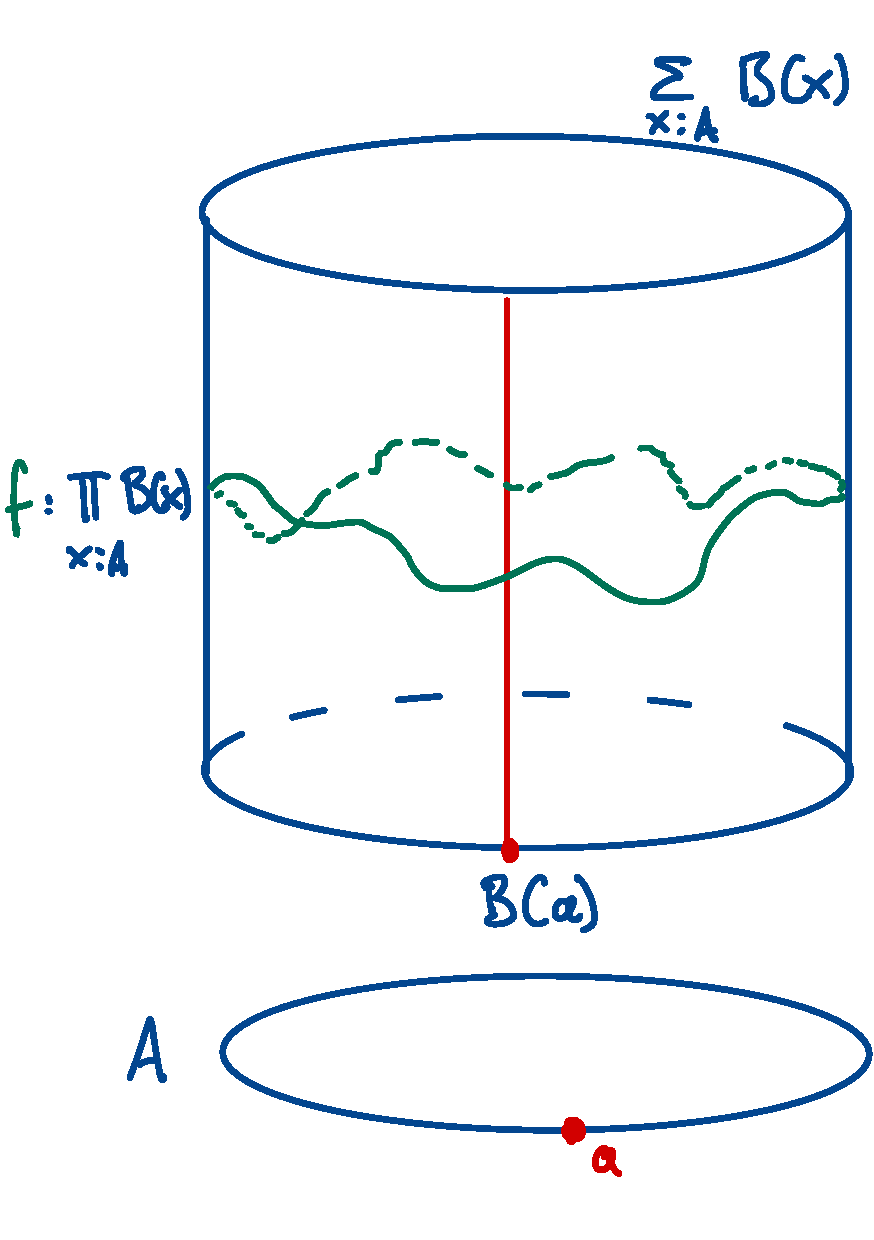
\includegraphics[width=\textwidth]{images/topology2.pdf}
        \end{column}%
    \end{columns}
\end{frame}

\begin{frame}{Weitere Typen -- mit homotopischer Interpretation}
    
    \begin{columns}[T] % align columns
        \begin{column}{.60\textwidth}
            \begin{itemize}
                \item Typfamilie $\Term{x} : \Type{A} \vdash \Type{B(x)}$ type $\leftrightsquigarrow$ Faserung über \Type{A}
                \item Dependent function Typ \Type{\prod_{x:A}B(x)} $\leftrightsquigarrow$ Raum der Schnitte
                
                Beispiel: \[\Term{\text{swap}}:\Type{\prod_{A:\Universe{}}\prod_{B:\Universe{}}\prod_{C:\Universe{}}(A\rightarrow B\rightarrow C)\rightarrow (B\rightarrow A\rightarrow C)}\]
            \end{itemize}
        \end{column}%
        \begin{column}{.30\textwidth}
            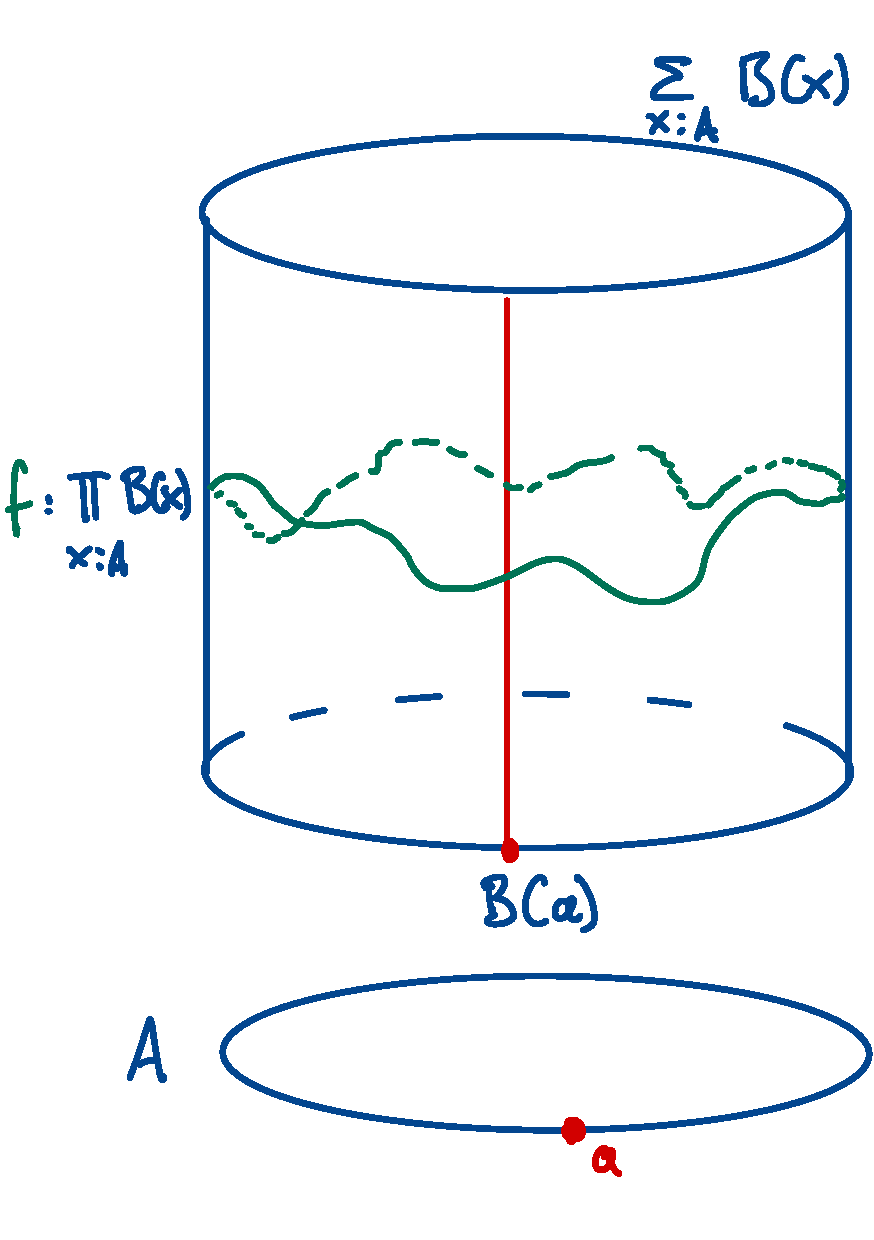
\includegraphics[width=\textwidth]{images/topology2.pdf}
        \end{column}%
    \end{columns}
\end{frame}

\begin{frame}{Kontrahierbare Typen}
    \begin{definition}{Kontrahierbare Typen}{}
        Es gibt einen eindeutigen Term vom Typ \Type{A} gdw.
        \[\Type{\sum_{a:A}\prod_{x:A} a=_{A}x}\]
        bewohnt ist, bzw. wenn der Raum \Type{A} \emph{kontrahierbar} ist.
    \end{definition}
\end{frame}

\begin{frame}{Typenäquivalenz}
    \begin{definition}{Typenäquivalenz}{}
        Zwei Typen \Type{A} und \Type{B} sind \emph{äquivalent}, wenn der Typ
        \[\Type{A\simeq B} :\equiv \Type{\sum_{f:A\rightarrow B}\left(\sum_{g:B\rightarrow A}\prod_{a:A}g(f(a))=_{A}a\right)\times\left(\sum_{h:B\rightarrow A}\prod_{b:B}f(h(b))=_{B}b\right)}\]
        bewohnt ist.
    \end{definition}
\end{frame}

\begin{frame}{Univalenzaxiom}
    Man kann leicht beweisen, dass
    \[\Type{(A = B) \rightarrow (A \simeq B)}.\]
    \begin{definition}{Univalenzaxiom (Voevodsky)}{}
        \[\Type{(A = B) \simeq (A\simeq B)}\]
    \end{definition}
\end{frame}

\begin{frame}{Der \glqq{}Stein von Rosette\grqq{} für HoTT}
    \begin{tabular}{l l l l}
        \toprule
        Typen & Logik & Mengen & Homotopie\\
        \midrule
        $\Type{A}$ & Aussage & Menge & Raum\\
        $\Term{a} : \Type{A}$ & Beweis & Element & Punkt\\
        $\Type{B(x)}$ & Prädikat & Mengenfamilie & Faserung\\
        $\Term{b(x)} : \Type{B(x)}$ & Bedingter Beweis & Elementfamilie & Schnitt\\
        $\Type{0}, \Type{1}$ & $\bot, \top$ & $\emptyset, \{\emptyset\}$ & $\emptyset, \star$\\
        $\Type{A + B}$ & $A\vee B$ & Disjunkte Vereinigung & Coprodukt\\
        $\Type{A \times B}$ & $A\wedge B$ & Menge von Paaren & Produktraum\\
        $\Type{A \rightarrow B}$ & $A\Rightarrow B$ & Menge von Funktionen & Funktionsraum\\
        $\Type{\sum_{(x:A)}B(x)}$ & $\exists_{x:A} B(x)$ & Disjunkte Summe & Totalraum\\
        $\Type{\prod_{(x:A)}B(x)}$ & $\forall_{x:A} B(x)$ & Produkt & Raum der Schnitte\\
        $\Type{\text{Id}_A}$ & Gleichheit ($=$) & $\{(x,x)\mid x\in A\}$ & Pfadraum $A^I$\\
        \bottomrule
    \end{tabular}
\end{frame}

\begin{frame}{Was gibt es noch?}
    \begin{itemize}
        \item HoTT und der $\lambda$-Kalkül
        \item Higher inductive types
        \item Beweistheorie in HoTT
    \end{itemize}
\end{frame}

\sectionslide{Anwendungen \& Aktuelle Forschungsfragen}

\begin{frame}{Anwendungen}
    \begin{itemize}
        \item Homotopietheorie
        \item Kategorientheorie
        \item Theorembeweiser
        \item Programmverifikation
        \item Funktionale Progammierung
    \end{itemize}
\end{frame}

\begin{frame}{Aktuelle Forschungsfragen}
    \begin{itemize}
        \item Informelle Typentheorie
        \item Formalisierung der klassischen Mathematik in HoTT
        \item Konstruktivität des Univalenzaxioms (Cubical Type Theory)
        \item HoTT auf diskreten Räumen (wie $\mathbb{N}$) führt zu vielen \glqq{}unnötigen\grqq{} Identitätstermen
        \begin{itemize}
            \item Möglichkeit, diese zu kollabieren
        \end{itemize} 
        \item HoTT und Topoi
        \begin{itemize}
            \item Intuitionistische Higher Order Logic ist die interne Sprache von $1$-Topoi, HoTT könnte die von $(\infty, 1)$-Topoi sein
        \end{itemize}
    \end{itemize}
\end{frame}

\begin{frame}[noframenumbering]{}
    \thispagestyle{empty}
    \begin{center}
        \scalebox{10}{\ucmark}
    \end{center}
\end{frame}

\begin{frame}{Aktuelle Forschungsfragen: Komplexitätstheorie?}
    \begin{itemize}
        \item Wenn HoTT Grundlage der Mathematik sein kann, muss man mit ihr auch Komplexitätstheorie betreiben können
        \item Klassische Komplexitätstheorie sehr \glqq{}mengenzentriert\grqq{}
        \item HoTT eng verbunden mit funktionalen Programmiersprachen
    \end{itemize}

    \begin{itemize}
        \item Mathematische Strukturen sind \glqq{}First Class Citizens\grqq{} in HoTT
        \begin{itemize}
            \item Codierung egal
        \end{itemize}
        \item Eher rekursionstheoretische Ansätze erforderlich~\cite{ctinctt}
        \begin{itemize}
            \item Maschinenunabhängige Komplexitätstheorie
            \item Implizite Komplexitätstheorie~\cite{icc}
        \end{itemize}
    \end{itemize}
\end{frame}

\begin{frame}{Aktuelle Forschungsfragen: Komplexitätstheorie?}
    \makebox[\textwidth][c]{\begin{tikzpicture}

        \draw[line width=7pt, maincolorMedium] (-2,0) -- (15,0);

        \fill (0.8, -0.2) rectangle (1.2, 0.2);
        \draw[-, line width=2pt] (1,-3) -- (1,0);
        \draw[align=center] (1, -3.5) node {Begriff der\\\glqq{}Linearität\grqq{} in HoTT$^\star$};


        \uncover<2->{\fill (4.8, -0.2) rectangle (5.2, 0.2);
        \draw[-, line width=2pt] (5,-4) -- (5,0);
        \draw (5, -4.5) node {Definition von Komplexitätsmaßen};}

        
        \uncover<3->{\fill (9.8, -0.2) rectangle (10.2, 0.2);
        \draw[-, line width=2pt] (10,-2) -- (10,0);
        \draw[align=center] (10, -2.5) node {Charakterisierung von sinnvollen\\Komplexitätsklassen und Hierarchien};}

        
        \uncover<4->{\fill (13.8, -0.2) rectangle (14.2, 0.2);
        \draw[-, line width=2pt] (14,-5) -- (14,0);
        \draw (9.5, -5.5) node {Charakterisierung von effizienter Berechenbarkeit~\cite{rtpoly}};}
    \end{tikzpicture}}~\\[2em]
    \tiny{$^\star$Danke an Prof. Thorsten Altenkirch~\cite{qtt1, qtt2}}
\end{frame}

\begin{frame}[standout]
    \Huge Danke!\\[2em]
    Fragen?
\end{frame}

\begin{frame}[allowframebreaks]
    \frametitle{Quellenverweise}
    \printbibliography[heading=none]
\end{frame}
    
\end{document}